\subsection{Styleguide für die Umsetzung}
Für ein einheitliches Erscheinungsbild der Webanwendung wurde in einem Styleguide definiert, welche Gestaltungsrichtlinen für die Entwicklung des Front-Ends gelten. 
Der Guide wurde den Front-End-Entwicklern zur Verfügung gestellt, damit 
sie diesen bei ihrer Entwicklung berücksichtigen können. 
In Abbildung \vref{fig:FE-StyleguideLogo} und \vref{fig:FE-StyColor} ist ein Auszug des Styleguides hinsichtlich des Logos und den einheitlichen Farben abgebildet.
Der vollständige Styleguide ist in Anhang \vref{an:Styleguide} einzusehen.
\begin{figure}[H]
	\centering 
	
\includegraphics[width=10cm]{img/FrontEnd/StyLogo.png}
	\caption[Auszug Styleguide für das Logo]{\label{fig:FE-StyleguideLogo}Auszug Styleguide für das Logo}
\end{figure}

\begin{figure}[H]
	\centering 
	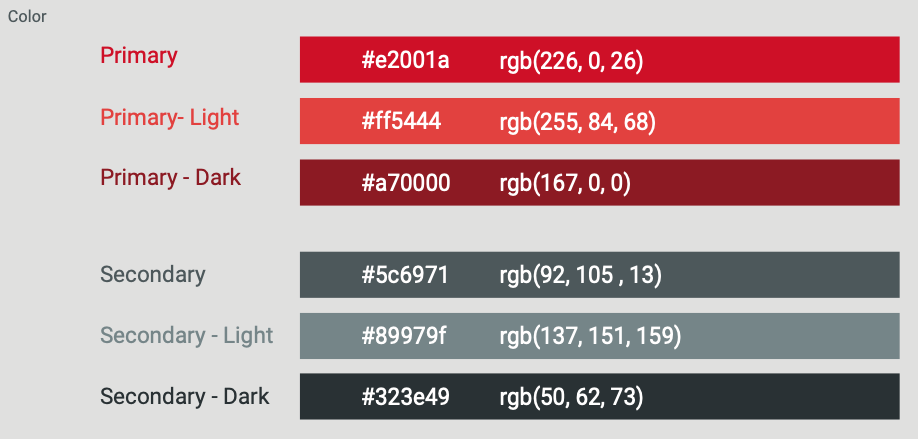
\includegraphics[width=10cm]{img/FrontEnd/StyColor.png}
	\caption[Auszug Styleguide für das Farbdesign]{\label{fig:FE-StyColor}Auszug Styleguide für das Farbdesign}
\end{figure}

\newpage
\subsection{Login}
Die Webanwendung startet gemäß der Anforderung A4 aus Tabelle \vref{anf:Profilzuordnung} mit einem Login, sodass sich der Benutzer anmelden oder registrieren kann. 
In Abbildung \vref{fig:FE-Login} ist die Login-Seite der Software zu sehen.
\begin{figure}[H]
	\centering 
	\includegraphics[width=\textwidth]{img/FrontEnd/Login.png}
	\caption[Login]{\label{fig:FE-Login}Login}
\end{figure}

\subsection{Kursübersicht}
Die Hauptansicht der Webanwendung ist die in Abbildung \vref{fig:FE-Vorlesungskalender} dargestellte Seite.
Hier werden die unterschiedlichen Kurse mit den jeweiligen Semestern, den Vorlesungen und dem eingebunden Kurskalendar angezeigt. 
Es können bereits angelegte Kurse verwaltet sowie neue Kurse angelegt werden. 
Die jeweiligen Vorlesungen können geplant werden, indem der aktuelle Stand der Vorlesungsorganisation mit der entsprechenden Dozentensuche angelegt wird.
In Unterkapitel \vref{ch:GC} wird die Einbindung des Kalendars sowie die Verbindung mit dem Google Calendar näher erläutert, da dies eine zentrale Komponente des Front-Ends darstellt.
\begin{figure}[H]
	\centering 
	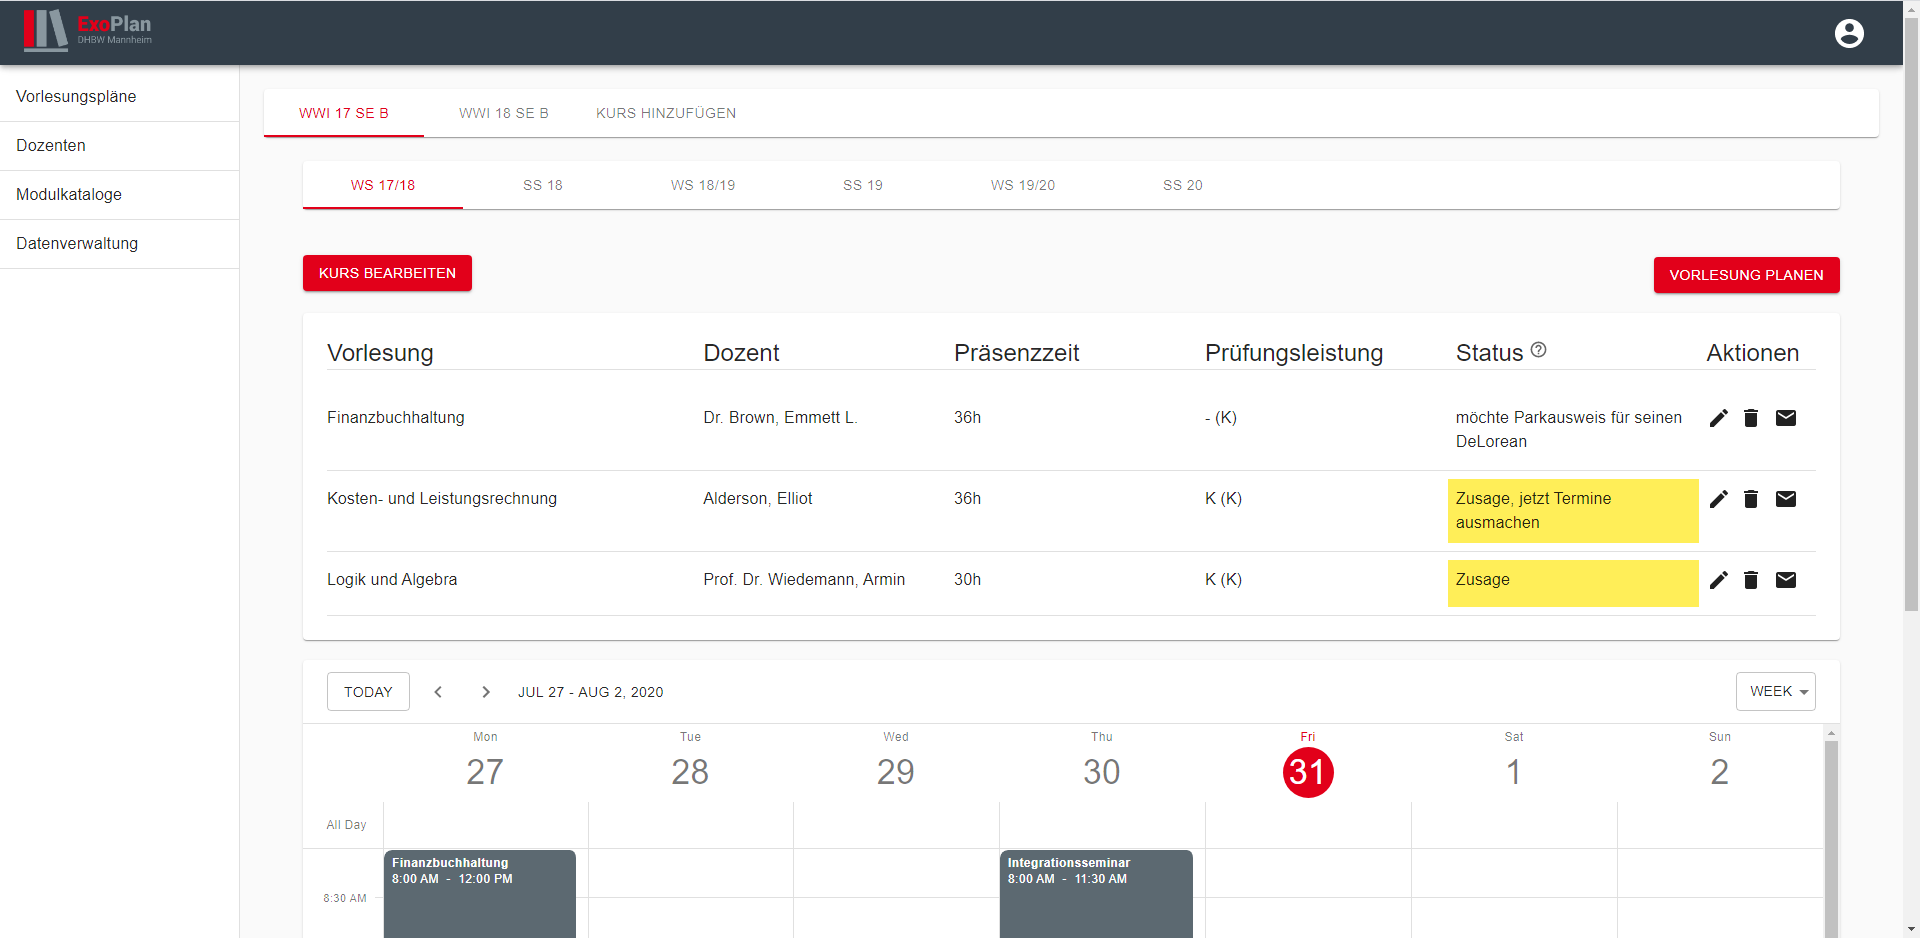
\includegraphics[width=\textwidth]{img/FrontEnd/Vorlesungskalender.png}
	\caption[Kursübersicht mit Vorlesungskalender]{\label{fig:FE-Vorlesungskalender}Kursübersicht mit Vorlesungskalender}
\end{figure}

\subsection{Dozentenansicht}
Unter dem Navigationspunkt \textit{Dozenten} wird der Dozentenpool dargestellt sowie die Möglichkeit zum Hinzufügen von neuen Dozenten gegeben.
Die Umsetzung der Anforderungen A1, A8, A9 und A12 aus Tabelle \vref{anf:Dozenten} ist in Abbildung \vref{fig:FE-Dozenten} zu sehen.
%In Abbildung \vref{fig:FE-DozentenDetail} ist 
Wird ein Dozent ausgewählt, erscheinen weitere Informationen in der Detail-Ansicht. Diese beinhaltet außerdem Funktionen, wie zum Beispiel das Hinterlegen eines Lebenslaufs.
\begin{figure}[H]
	\centering 
	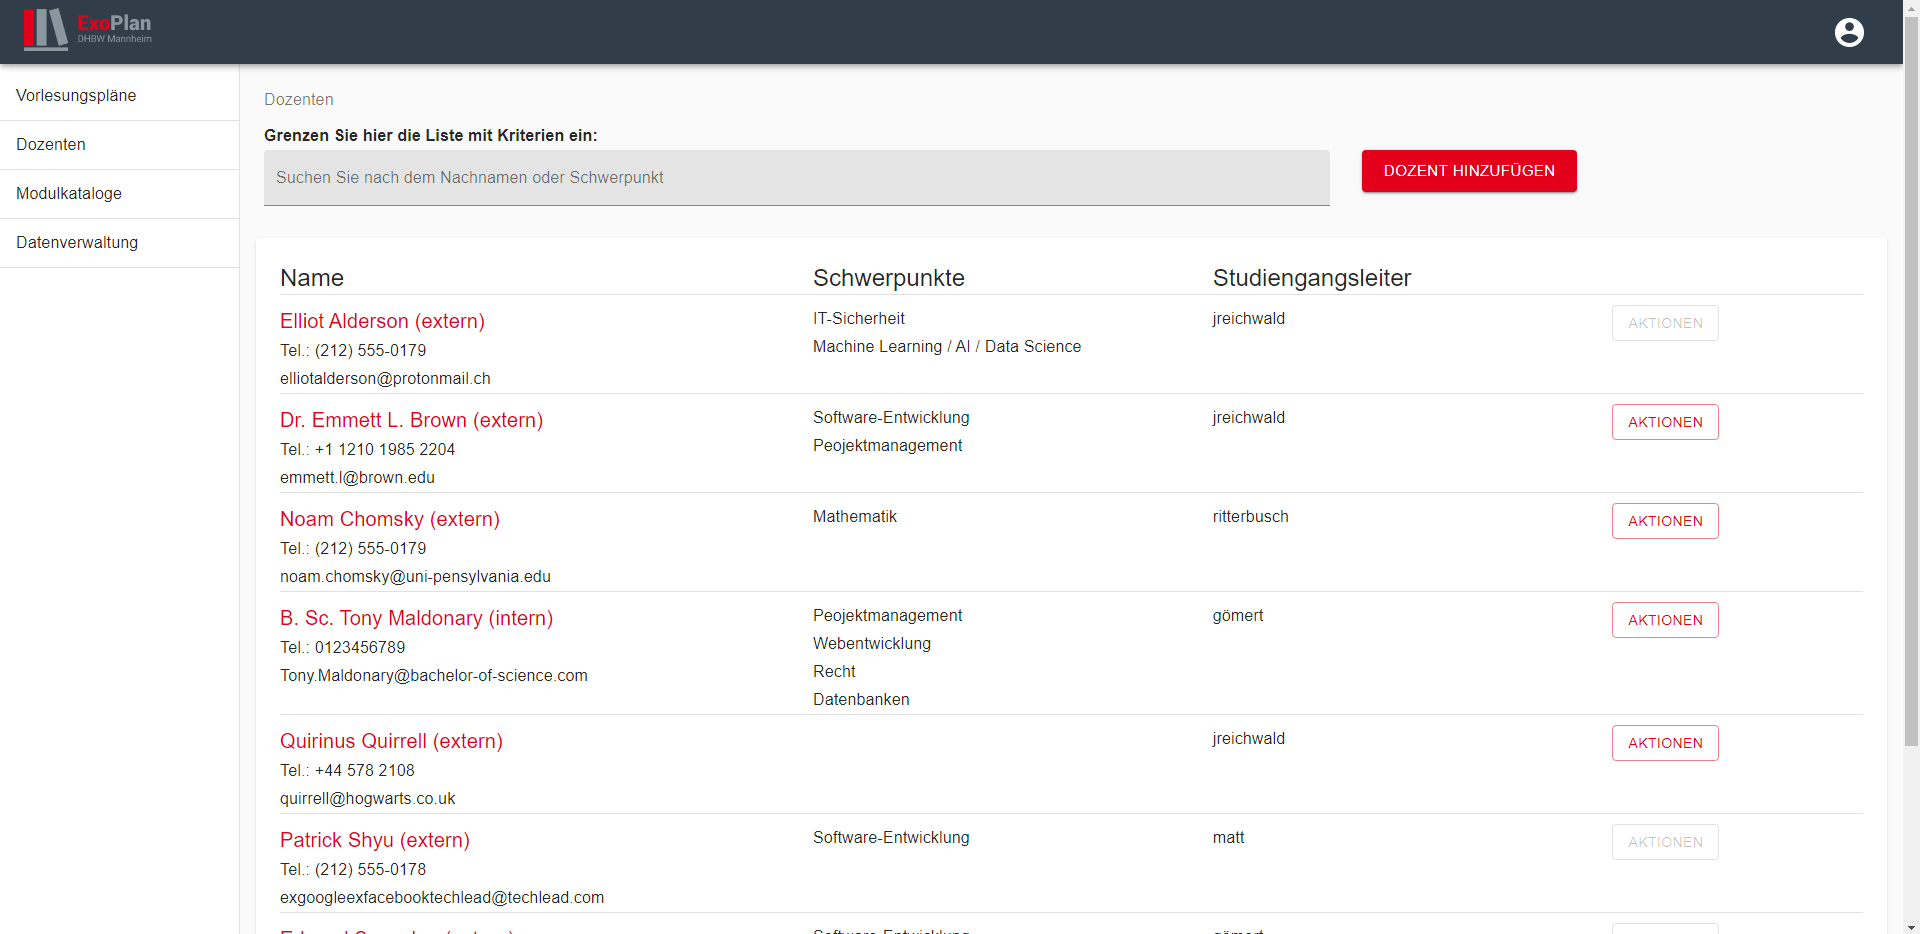
\includegraphics[width=\textwidth]{img/FrontEnd/Dozenten.png}
	\caption[Anzeige der Dozenten]{\label{fig:FE-Dozenten}Anzeige der Dozenten}
\end{figure}
%\begin{figure}[H]
%	\centering 
%	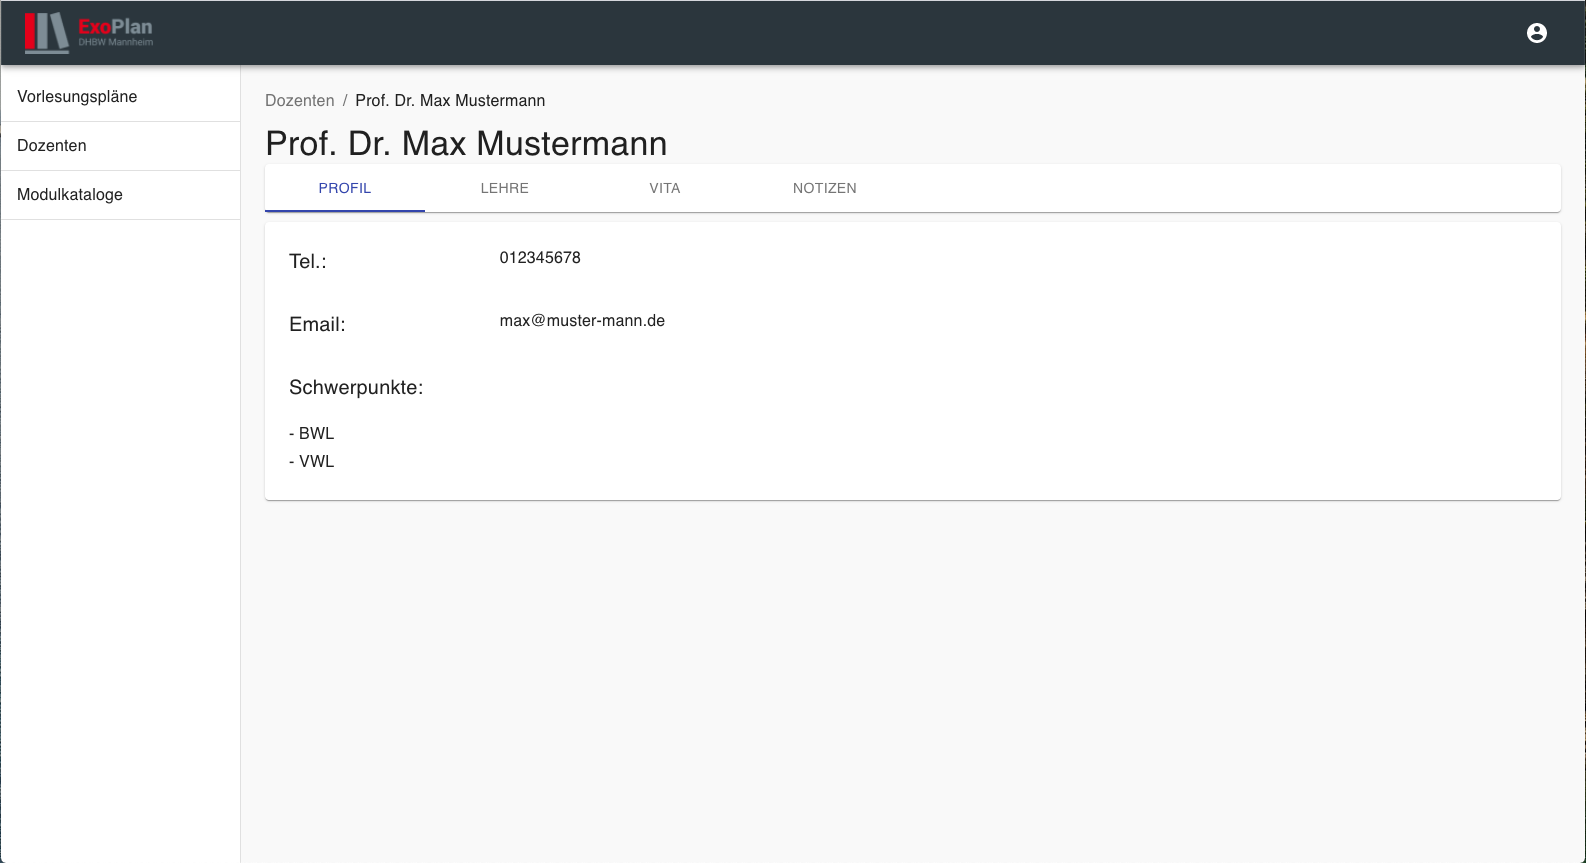
\includegraphics[width=\textwidth]{img/FrontEnd/DozentDetail.png}
%	\caption[Anzeige eines Dozenten]{\label{fig:FE-DozentenDetail}Anzeige eines Dozenten}
%\end{figure}

\subsection{Modulkatalog}
Mit dem Navigationspunkt \textit{Modulkatalog} wird die Anforderungen A4 aus Tabelle \vref{anf:Modulkatalog} umgesetzt. 
Es können Modulkataloge hinzugefügt, angezeigt sowie verwaltet werden. 
\begin{figure}[H]
	\centering 
	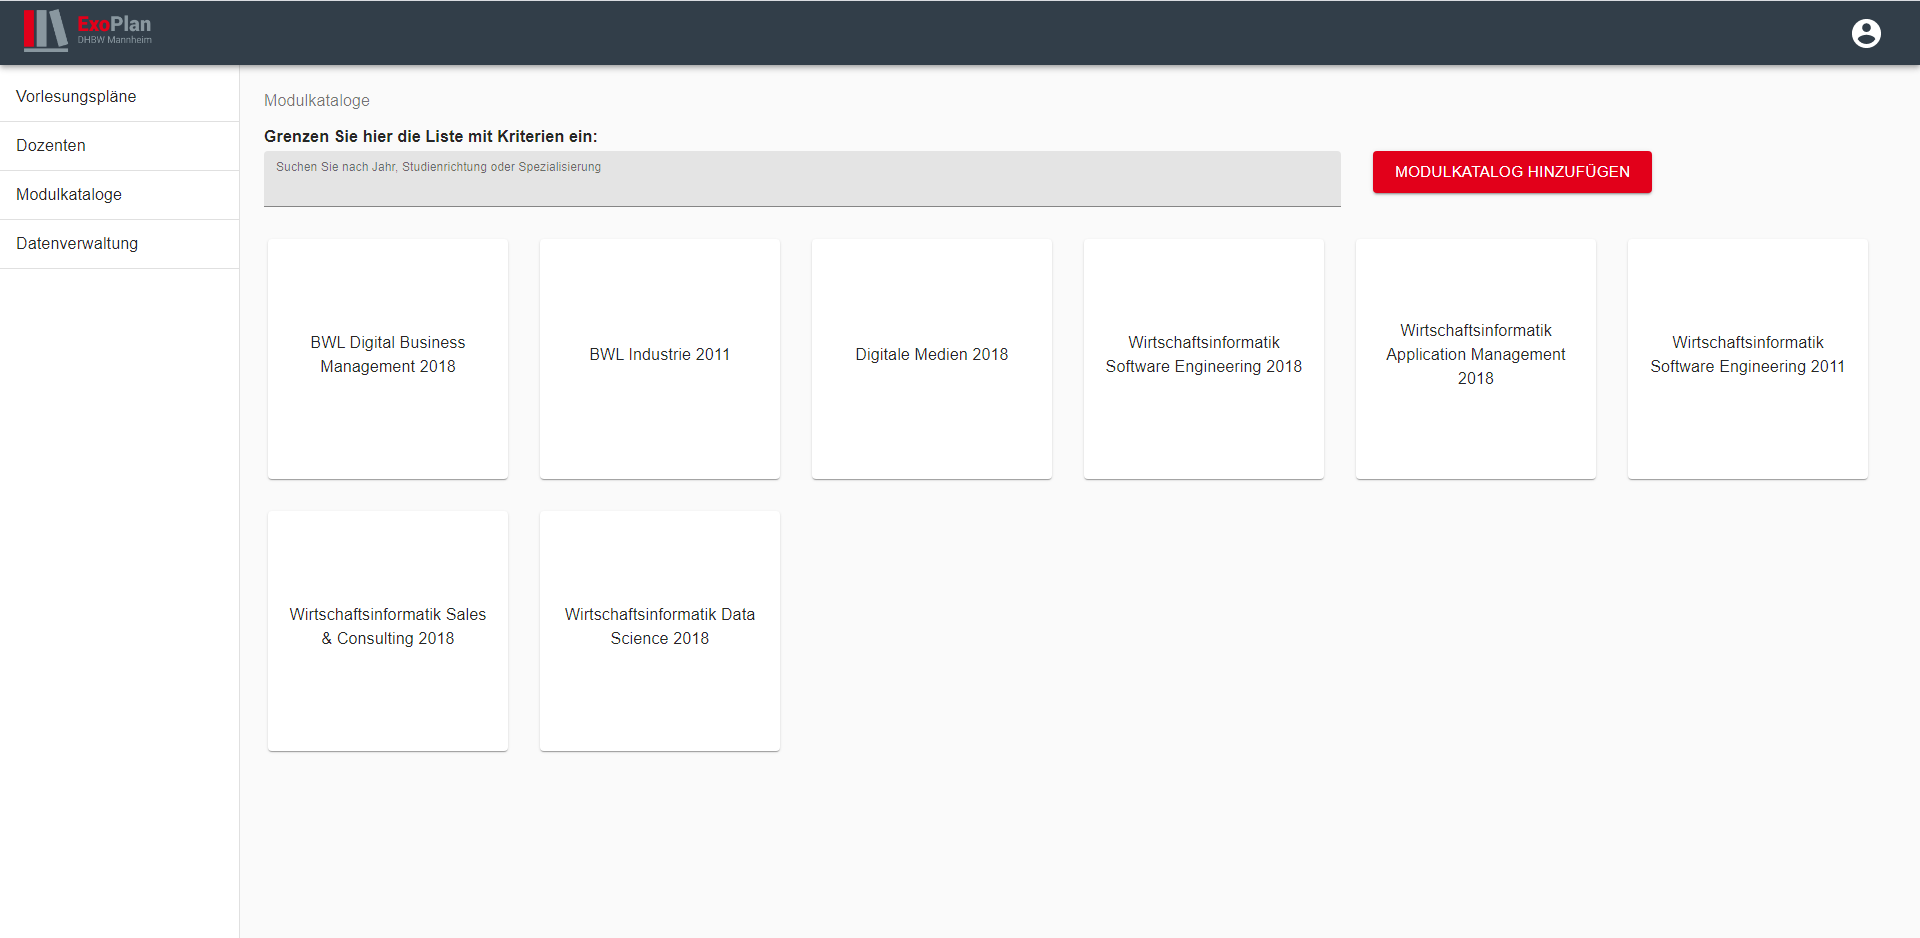
\includegraphics[width=\textwidth]{img/FrontEnd/Modulkataloge.png}
	\caption[Anzeige der Modulkatalogen]{\label{fig:FE-Modulkataloge}Anzeige der Modulkatalogen}
\end{figure}

\subsection{Datenverwaltung}
In der Datenverwaltung können die Studiengänge, die Schwerpunkte sowie die Prüfungsleistungen verwaltet werden.
In Abbildung \vref{fig:FE-Datenverwaltung} ist das Hinzufügen, Bearbeiten und Löschen von Studiengängen abgebildet.
\begin{figure}[H]
	\centering 
	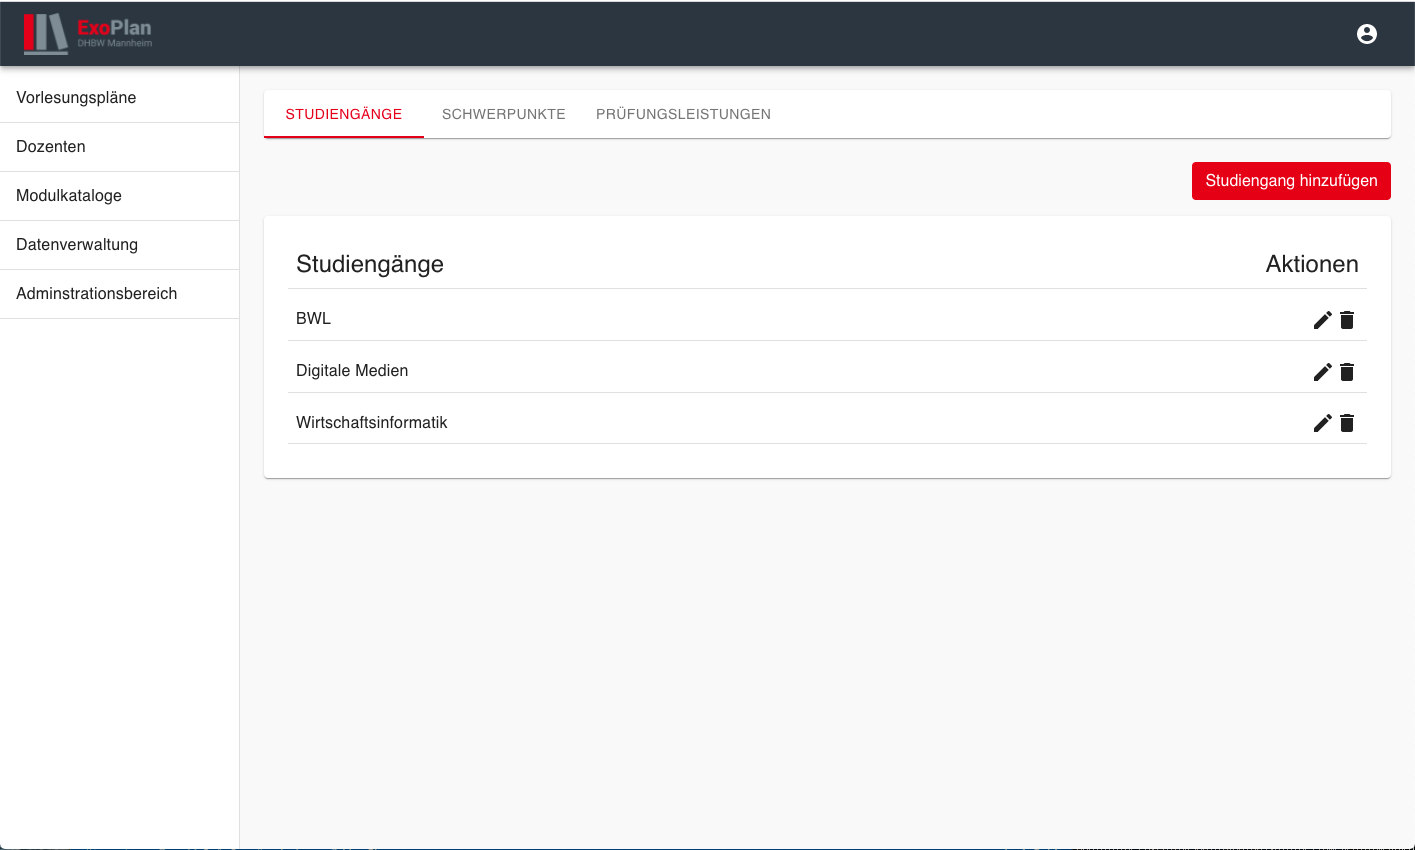
\includegraphics[width=\textwidth]{img/FrontEnd/Datenverwaltung.png}
	\caption[Datenverwaltung]{\label{fig:FE-Datenverwaltung}Datenverwaltung}
\end{figure}

\subsection{Administrationsbereich}
Der Administrationsbereich erlaubt es Nutzern mit der Benutzerart \textit{Administrator} andere Benutzer zu verwalten.
Neben dieser Funktionalität, in Abbildung \vref{fig:FE-Administrationsbereich} dargestellt, können Registrierungsschlüssel sowie der Zugang zu dem Google Calendar verwaltet werden.
\begin{figure}[H]
	\centering 
	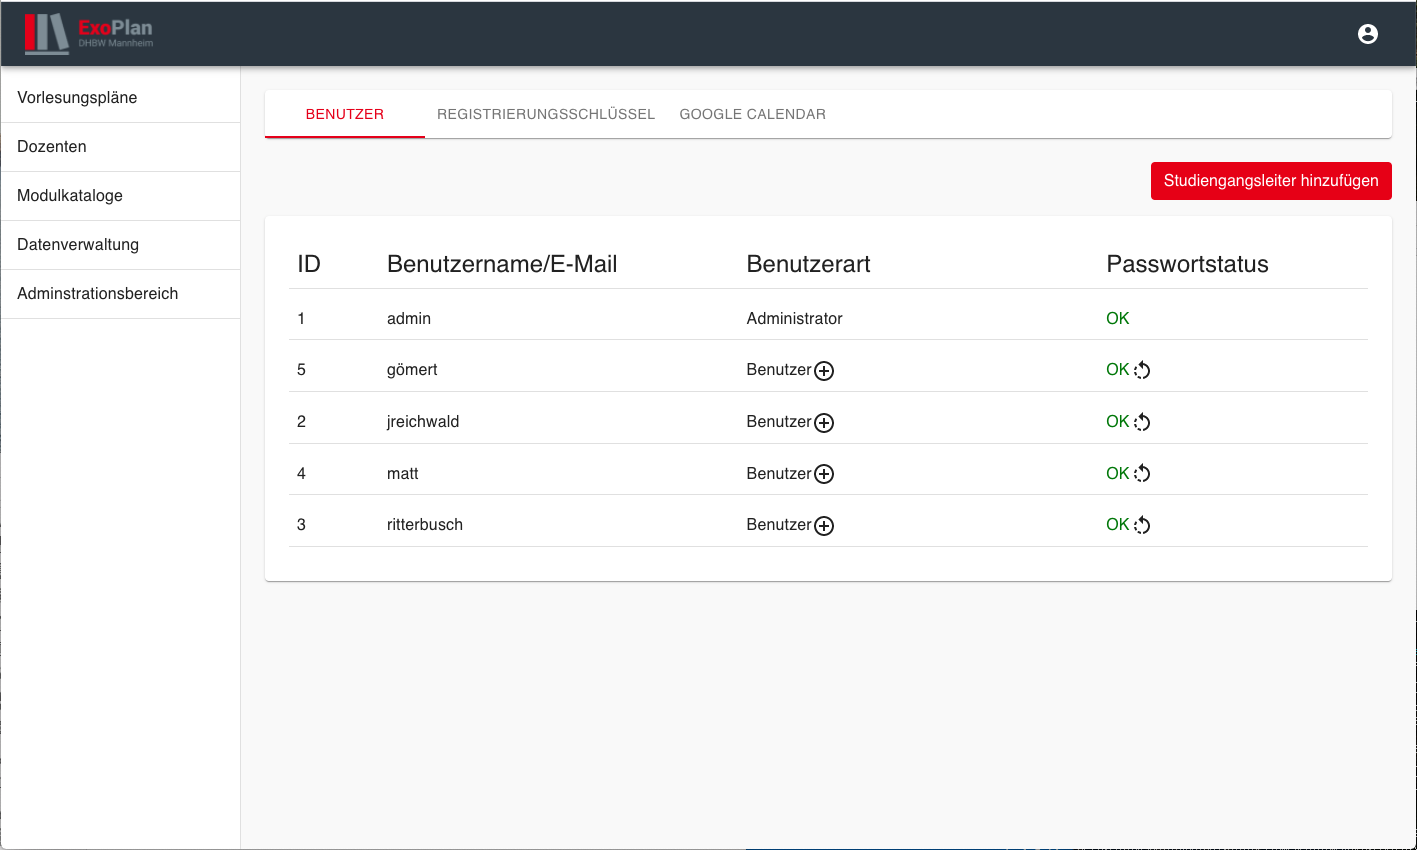
\includegraphics[width=\textwidth]{img/FrontEnd/Administrationsbereich.png}
	\caption[Administrationsbereich]{\label{fig:FE-Administrationsbereich}Administrationsbereich}
\end{figure}

\subsection{Allgemeine Einstellungen}
Zusätzlich können allgemeine Einstellungen für den Benutzer des Profils verändert werden, die in Abbildung \vref{fig:FE-Einstellungen} dargestellt sind.
So kann der Benutzer unter anderem sein Passwort ändern.
\begin{figure}[H]
	\centering 
	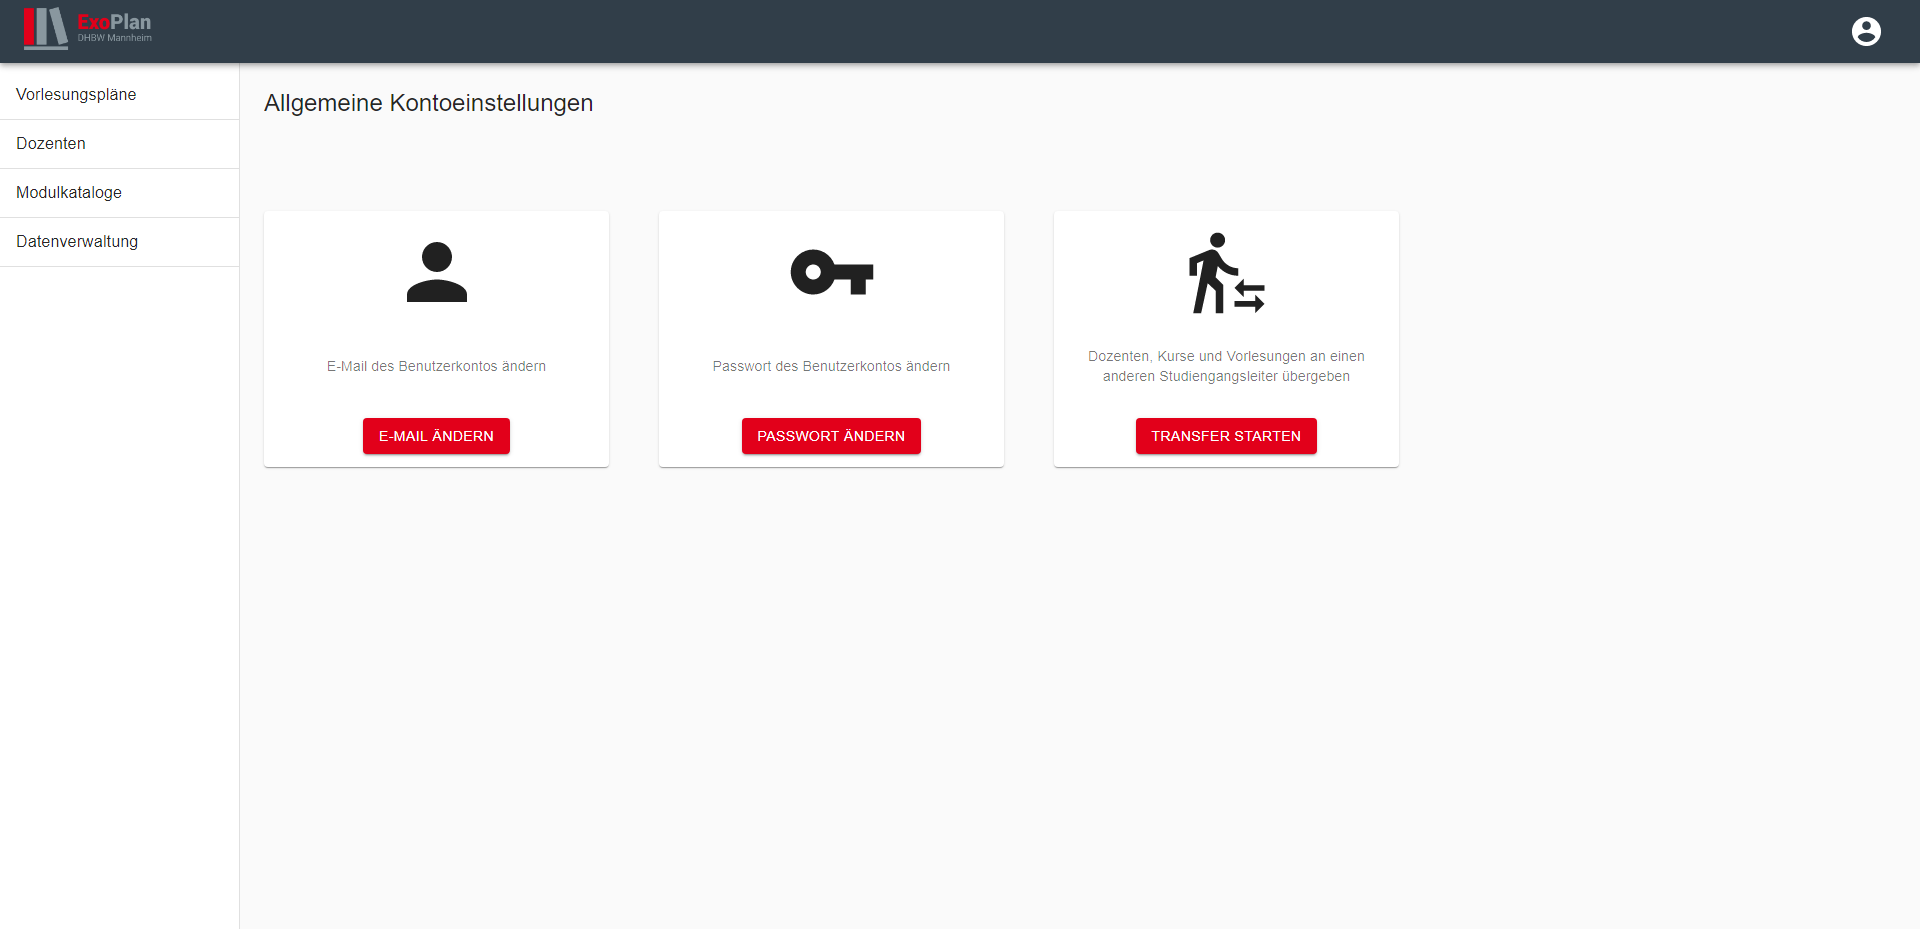
\includegraphics[width=\textwidth]{img/FrontEnd/Einstellungen.png}
	\caption[Allgemeine Kontoeinstellungen]{\label{fig:FE-Einstellungen}Allgemeine Kontoeinstellungen}
\end{figure}
